%%%%%
%%Title: HiPi+Bus V0.2 Chapter 7
%%Creator: Ando Ki
%%CreationDate: April 1992
%%FileName: sec4
%%RelatedFile: ch7
%%%%%
\section{BTL 신호의 전기적 규격}
BTL의 정확한 규격은 IEEE Std.1194.1을 따른다. \\
%
BTL 신호의 전기적 규격은 {\tt <}표~\ref{table:btl-spec}{\tt >}와 같다.
%
%
\begin{table}[htbp]
\caption{BTL 신호의 전기적 규격}\label{table:btl-spec}
   \begin{center}
   \begin{tabular}{|l l|l|} \hline
	$V_t$    & typical & 2.0V\\
	$V_{OH}$ & min     & 1.9V\\
	$V_{IH}$ & min     & 1.62V\\
	$V_{IL}$ & max     & 1.47V\\
	$V_{OL}$ & max     & 1.1V\\
	$V_{OL}$ & min     & 0.75V\\
	$GND$    &         & 0.0V\\ \hline
   \end{tabular}
   \end{center}
\end{table}
%

%
신호의 참조전압을 GND 0V라 하고, 터미네이션에 의한 전압이 $V_t$이고,
신호가 구동되지 않은 상태에서의 신호선의 전압은 $V_{OH}^{min}$ 이상이 되어야 하고,
신호선에 신호를 구동할 때 구동소자는 해당 신호선의 전압을 $V_{OL}^{max}$와
$V_{OL}^{min}$ 사이가 되도록 해야 한다.
수신소자의 경우는 $V_{IH}^{min}$ 이상이 되는 전압에 대해서는 높은 전압으로,
$V_{IL}^{max}$ 이하의 전압에 대해서는 낮은 전압으로 받아들여야 한다.
이것을 그림으로 나타내면 {\tt <}그림~\ref{figure:signal-spec-btl}{\tt >}과 같다.
%
\begin{figure}[htb]
    \centerline{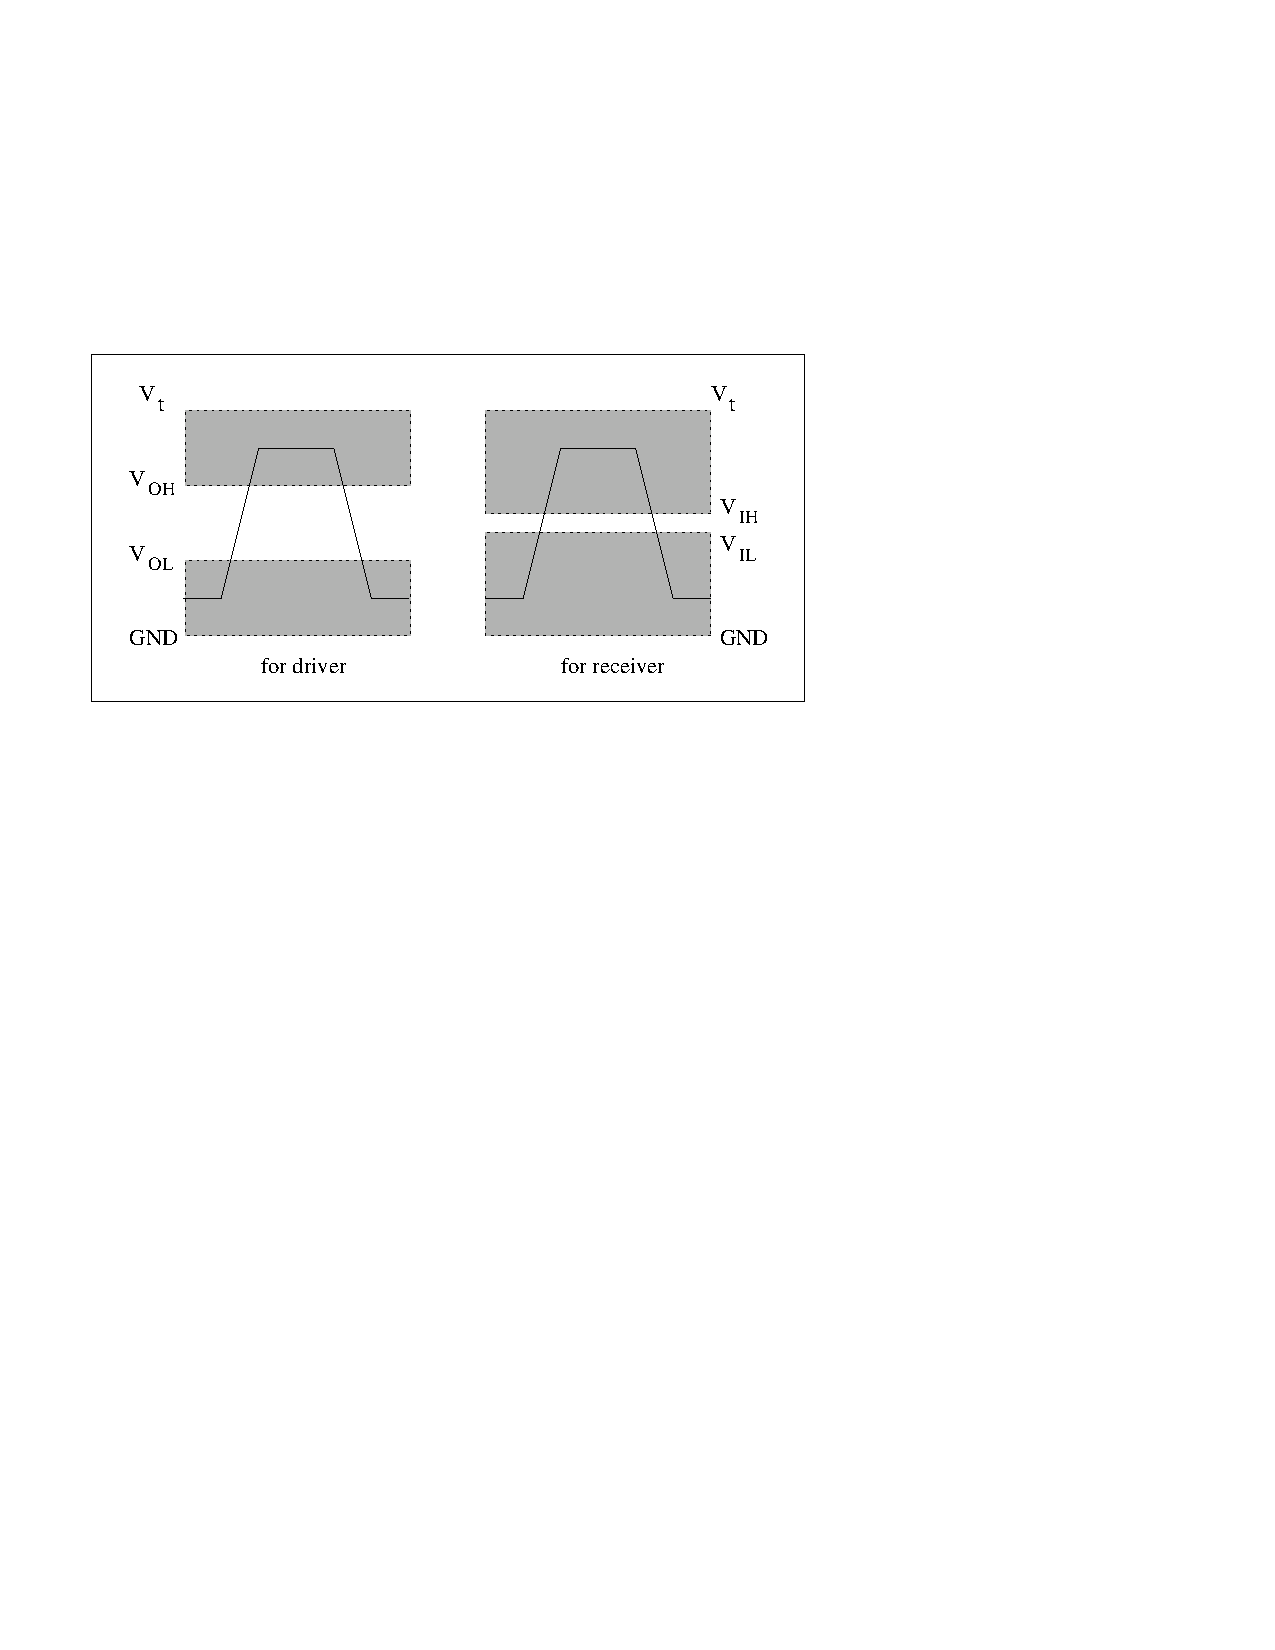
\includegraphics{ch7/FIG/signal-spec.jpg}}
   \caption{BTL 신호선의 전기적 규격}\label{figure:signal-spec-btl}
\end{figure}
%

\subsection{인터페이스 회로의 용량성 부하}
%
BTL 버스에 연결되는 수신소자(receiver), 구동소자(driver), 수신/구동소자(transceiver)의
각 출력단의 용량성 부하는 5$p$F보다 크지 않아야 한다.

\subsection{인터페이스 회로의 누설 전류}
%
백플레인 신호선의 전압이 $V_{OL}$ 영역에 있을때,
해당 신호선에 연결된 인터페이스 소자중 신호를 구동하지 않는 소자의 역방향 누설 전류(negative
leakage current)가 $-250\mu A$보다 작아야 한다.
즉 최대 역방향 누설 전류(maximum negative leakage current)가
$-250\mu A$이다.\\
백플레인 신호선의 전압이 $V_{OH}$ 영역에 있을때,
해당 신호선에 연결된 인터페이스 소자는 제~\ref{sec:voh}장에서 규정하는
최대 순방향 누설 전류(maximum positive leakage current)를 보장해야 한다.

\subsection{구동소자}
%
\subsubsection{구동소자 형태}
%
구동소자는 낮은 전압이 참이어야만 하고, wired-OR 기능이 있어야만 한다.

\subsubsection{정적 부하 전류 (static load current)}
%
백플레인 신호선의 전압이 $V_{OL}$ 일때 구동 소자는 80$m$A의 전류 흡수능력(current
sinking capability)이 있어야 한다.

\subsubsection{구동소자의 $V_{OH}$}\label{sec:voh}
%
$V_{OH}$는 누설 전류, 터미네이션 전압, 부하저항, 그리고 백플레인에 연결된 소자의 수에 의해
결정된다. $V_{OH}^{min}$는 1.9V 이며, 이것은 식 (\ref{eqn:vol})에 의해
정의된다. $V_{OH}^{max}$는 누설 전류가 없는 상황에서 터미네이션 전압 $V_t$가 된다.
%
\begin{table}[htb]
  \begin{eqnarray}
	V_{OH}^{min} & = & V_t - \frac{n \times I_l}{2}
		\times R_t \label{eqn:vol}
  \end{eqnarray}
%
   \begin{center}
   \begin{tabular}{ll}
	$V_t$ & : the termination voltage\\
	$I_l$ & : the maximum positive leakage current\\
	$n$   & : the number of devices on the bus
		(assuming all have the same $I_l$\\
	$R_t$ & : the termination resistor\\
   \end{tabular}
   \end{center}
\end{table}
%

\subsubsection{구동소자의 $V_{OL}$}
%
구동소자의 $V_{OL}$은 전류 흡수가 80$m$A일때 0.75V에서 1.1V사이를
유지해야만 한다.

\subsubsection{천이시간 (transition times)}
%
10\%에서 90\%로의 상승 시간과 90\%에서 10\%로의 하강 시간은 10$n$sec보다
크지 않아야 한다. 그리고 잡음을 최소화하기 위해서는 구동소자가 출력 천이 시간을 3$n$sec보다
작지 않게 해야한다.

\subsection{수신소자}
%
\subsubsection{임계영역 (threshold)}
%
백플레인 신호선에 연결된 모든 수신소자의 수신 임계영역 전압(receiver threshold
voltage)은 엄격히 지켜져야 한다. 1.47V 이하인 경우는 낮은 전압으로,
1.62V이상이면 높은 전압으로 규정한다.
앞에서 규정한 좁은 임계영역전압을 보장함으로써 높은 잡음 허용한계를 얻을 수 있다.

\subsubsection{잡음제거 (noise rejection)}
%
잡음의 영향을 최소화 하기 위해 3$n$sec 미만의 펄스를 제어하는 필터를 수신측에 허용한다.

\subsubsection{입력 클램퍼 (input clamps)}
%
과도한 역저압에 의한 영향을 방지하기 위해 1.5V에 적어도 12$m$A의 클램핑 회로가
수신소자의 입력단에 있어야 한다.
%%%%%
%\end{document}
%%%%%
